\chapter{Implementation}
\label{chap:implementation}

\section{Requirements}
    % List and explain the requirements from the specialisation project.
    In the specialisation project leading up to this master's thesis, functional and non-functional requirements were identified. They have been slightly improved in this master's thesis to be clearer and more specific, and one new non-functional requirement (\textbf{nFR6}) have been added explicitly.
    
    \FloatBarrier
    \begin{table}
    \label{tab:fr}
    \caption{Functional Requirements}
    \begin{tabular}{ | c | p{0.9\linewidth} | }
        \hline
        \textbf{ID} & \textbf{Description} \\
        \hline
        FR1 & The Virtual Field Trip (VFT) shall feature a landscape around Vekveselva reconstructed from LiDAR data. \\
        FR2 & The VFT shall use the Virtuix Omni Omnidirectional Treadmill and the HTC Vive Pro Head Mounted Display. \\
        FR3 & The VFT landscape shall have flat areas that the user can walk on.\\
        FR4 & The VFT shall have the ability to transition between a virtual landscape and footage from the real area. \\
        FR5 & The VFT shall project footage either onto spheres or onto the ground, using shaders. \\
        FR6 & The VFT shall contain tasks relevant to the field trip that the player can perform. \\
        FR7 & The VFT shall have a menu where the application can be started, restarted and exited. \\
        \hline
    \end{tabular}
    \end{table}
    \FloatBarrier
    
    \FloatBarrier
    \begin{table}
    \label{tab:nfr}
    \caption{non-Functional Requirements}
    \begin{tabular}{ | c | p{0.9\linewidth} | }
        \hline
        \textbf{ID} & \textbf{Description} \\
        \hline
        nFR1 & The application shall offer at least three of Lazzaro's four fun keys. \\
        nFR2 & The application shall have tasks with intuitive interaction. \\
        nFR3 & The application shall be engaging. \\
        nFR4 & The application shall be fun. \\
        nFR5 & The application shall have good performance, keeping the framerate high enough to not be uncomfortable. \\
        nFR6 & The application shall be based on open source software and tools. \\
        \hline
    \end{tabular}
    \end{table}
    \FloatBarrier

\section{Minimal Viable Product}
    % A prioritised list of features to be implemented. The first points are regarded as minimum to be completed. Create the list together with domain experts and supervisor.
    The development technique for creating the new Oppdal Application is the Minimal Viable Product (MVP) approach. Techopedia\cite{techopedia} defines this at the technique where a product is developed containing the bare minimum functionality. Then, more features are added, typically through feedback produced by the MVP. This technique has two major benefits for this master's thesis. Firstly, it allows users to be included as early as possible in order to better guide the product from an early part of the development when changes are less cumbersome to make. Secondly, it allows for more dynamic planning, as the developer is less experienced in the tools and frameworks necessary to develop the application. This is likely to result in less time used for planning and re-planning due to the uncertainty in time estimates. The plan for the MVP is a prioritised list as can be seen below. The line separates the ''must-have'' features of the MVP from the ''if-time'' features that can be added.
    
    \todo{Write more about development methodology}
    
    \setcounter{rownumbers}{0}
    
    \FloatBarrier
    \begin{table}
    \label{tab:mvp}
    \caption{Prioritised List of Features for the Application}
    \begin{tabular}{@{\stepcounter{rownumbers} \therownumbers\hspace*{\tabcolsep}} p{0.9\linewidth}}
        Recreate topology from LiDAR \\
        Re-texture topology \\
        Decorate area with prefabs of trees and grass \\
        Incorporate existing image viewer for 360 VR images \\
        Implement a menu for starting and exiting the application \\
        Implement game mechanic (\emph{to be discussed exactly what}) \\
        \hline
        Convert image viewer from plateau to spheres and texture either them or the surroundings with the images (\emph{to be discussed - is it necessary / prioritised?}) \\
        Implement more game mechanics \\
        Improve prefab decorations of the area
    \end{tabular}
    \end{table}
    \FloatBarrier
    
    \todo{Update with latest agreed list from domain expert}

\section{Development Plan}
    % Create a time table with milestones
    To keep tab of the progress, the following development plan with milestones was used:
    
    \FloatBarrier
    \begin{table}
    \label{tab:plan}
    \caption{Plan with Milestones for the Project}
    \begin{tabular}{| p{0.2\linewidth} | p{0.725\linewidth} |}
        \hline
        \textbf{Time} & \textbf{Milestone} \\
        \hline
        End of January & Finalise the shape of the terrain and finish the MVP feature list \\
        End of February & Finish decorating the area with prefabs, incorporate image viewing and decide on game mechanics to be used in cooperation with domain experts \\
        End of March & Implement game mechanics \\
        14th of April & Finish prototype development and freeze code. Finish questionnaires for testing and tasks for the Penn State application. \\
        End of April & Finish user testing with students and finish interview questions for domain experts \\
        End of Mai & Finish user testing, interviewing domain experts and finish comparison of applications \\
        10 of June & Finish structuring and analyse collected data, finalise the project and the report \\
        \hline
    \end{tabular}
    \end{table}
    \FloatBarrier

\section{Creating the Ground Model}
    % Kartverket    - acquire point cloud
    % LasTools      - merge files
    % LasTools      - filter vegetation
    % LasTools      - convert to .txt
    % Meshlab       - import .txt
    % Meshlab       - recreate normals  (normal recreation)
    % Meshlab       - recreate topology (screened poisson surface)
    % Meshlab       - simplify          (MC edge collapse)
    % Meshlab       - cleaning          (remove duplicate vertices and faces)
    % Meshlab       - set origin        (transform, set origin)
    % Meshlab       - export .ply
    % Blender       - import .ply       (viewport must be adjusted)
    % Blender       - cut model         (Blender nearly crashes at this point, loads unresponsive for 20+ seconds, not done in Meshlab because want other than square regions)
    % Blender       - export .ply
    % Meshlab       - import .ply
    % Meshlab       - simplify          (quadratic edge collapse decimation 0.01 on area and 0.001 on surroundings)
    % Meshlab       - export .ply
    % Blender       - import .ply
    % Blender       - rework walkway    (curve, box, edit box, array box, curve box, shrinkwrap)
    % Blender       - texture models    (materials, image brush)
    % Blender       - export .fbx and texture image
    % Unity         - import .fbx and texture image
    As explained more in detail in the Specialisation Project\cite{specialisation}, the topology has been recreated from LiDAR scanning of the area, publicly available at Kartverket\cite{hoydedata}. The complete pipeline for creating a usable model for the ground without sacrificing too much performance is a long and iterative one. In order to get an overview of the process, as well as details and reasoning, the entire pipeline is presented as a numbered list in \cref{tab:pipeline}, followed by sections detailing the steps. The numbered list also contains a column showing which software or service is used in each step.
    
    \setcounter{rownumbers}{0}
    
    \FloatBarrier
    \begin{table}[htbp]
        \centering
        \caption{Reconstruction Pipeline Steps}
        \label{tab:pipeline}
        \begin{tabular}{| c | c | p{0.575\linewidth} |}
            \hline
            \textbf{Number} & \textbf{Software / Service} & \textbf{Description} \\
            \hline
            \rownumber & Kartverket\footnote{The Norwegian Mapping Authority} & Acquire point cloud in \texttt{.laz} files \\
            \rownumber & LasTools & Merge the \texttt{.laz} files into one \\
            \rownumber & LasTools & Filter out the vegetation from the \texttt{.laz} files \\
            \rownumber & LasTools & Convert \texttt{.laz} file to \texttt{.txt} file \\
            \rownumber & Meshlab & Recreate normals for points \\
            \rownumber & Meshlab & Recreate surface \\
            \rownumber & Meshlab & Simplify (decimation) and cleaning \\
            \rownumber & Meshlab & Set origin \\
            \rownumber & Meshlab & Export model as \texttt{.ply} file \\
            \rownumber & Blender & Cut model into smaller parts\\
            \rownumber & Blender & Export models as \texttt{.ply} files \\
            \rownumber & Meshlab & Simplify (decimation) and cleaning \\
            \rownumber & Meshlab & Export models as \texttt{.ply} files \\
            \rownumber & Blender & Rework walkway model \\
            \rownumber & Blender & Texture models \\
            \rownumber & Blender & Export models as \texttt{.fbx} files \\
            \hline
        \end{tabular}
    \end{table}
    \FloatBarrier
    
    \subsection{Acquire Point Cloud from Kartverket}
        The first step of creating the ground model is to acquire the LiDAR scanning of the area. The scanning is openly available at the Norwegian Mapping Authority - Kartverket. On their web pages, the area in question can be marked and the data files will be made available at a custom link address. Depending on the size of the area, the data will typically be divided into several \texttt{.laz} files.
        
        It could also be possible to get terrain models directly from Kartverket. One would then have to find software to open the model files (\texttt{geoTiff}) and find another way to filer out the vegetation.
    
    \subsection{Filter with LasTools}
        LasTools\cite{lastools} is a semi-open source software developed by rapidlasso. It has several functions to work on point cloud data, where some are completely open source, and others are free to use for non-commercial projects.
        
        With the \texttt{.laz} files available, the most practical thing is to merge the files into one. Afterwards, the terrain can be filtered from the vegetation using one of the only-for-non-commercial functions: \texttt{lasground\_new.exe}. Finally, the point cloud can be exported as a \texttt{.txt} file that Meshlab can read.
    
    \subsection{Reconstruct Surface with Meshlab}
        The software used for the surface recreation is Meshlab\cite{LocalChapterEvents:ItalChap:ItalianChapConf2008:129-136}. It is open source and made for working with large point clouds and models, as well as supporting mesh reconstruction. Although it could be a good idea to reduce the size of the point cloud, the model contains a walkway in the valley that is important to keep as precise as possible.
        
        \FloatBarrier
        \begin{figure}[htbp]
            \centering
            \includegraphics[width=\ImageWidth]{figures/point_cloud.PNG}
            \caption{Filtered Point Cloud for the Ground in the Vekveselva River Area}
            \label{fig:point_cloud}
        \end{figure}
        \FloatBarrier
        
        Screened Poisson Surface Reconstruction\cite{kazhdan2013screened} was used to recreate the ground model from the point cloud. It relies on the points having normals, so these normals had to be calculated first. The reconstructing algorithm was tested with different reconstructing depths where the choice landed on 12. This resulted in longer computing time but a very good reconstruction quality. The model was also cleaned for duplicate edges and vertices without normals.
        
        Because the ground model is constructed from points, and the points have gps coordinates, the resulting model has a very large offset from its local origin. Although a better practise would be to keep these coordinates, as they could be useful information later, they made it hard to locate the model in programs like Blender. Therefore the origin of the model was reset to approximately the centre of the geometry. The model was exported as a \texttt{.ply} file as it can be read by both Blender and Meshlab and has good compression.
    
    \subsection{Cut Model in Blender}
        Blender\cite{blender} is a versatile, open source software with many different features. It was used to further rework and texture the model where Meshlab proved less appropriate. It was first used to partition the model into three smaller areas that would be simplified at different rates. This partitioning can be seen in \cref{fig:model_original}. The reasoning behind the partition is to cut the model into the part that the player will move on, the are they will look at most, and the part they are only supposed to view at a distance or not at all. This will also allow parts of the model to be worked on in isolation from the rest.
        
        \FloatBarrier
        \begin{figure}[htbp]
            \centering
            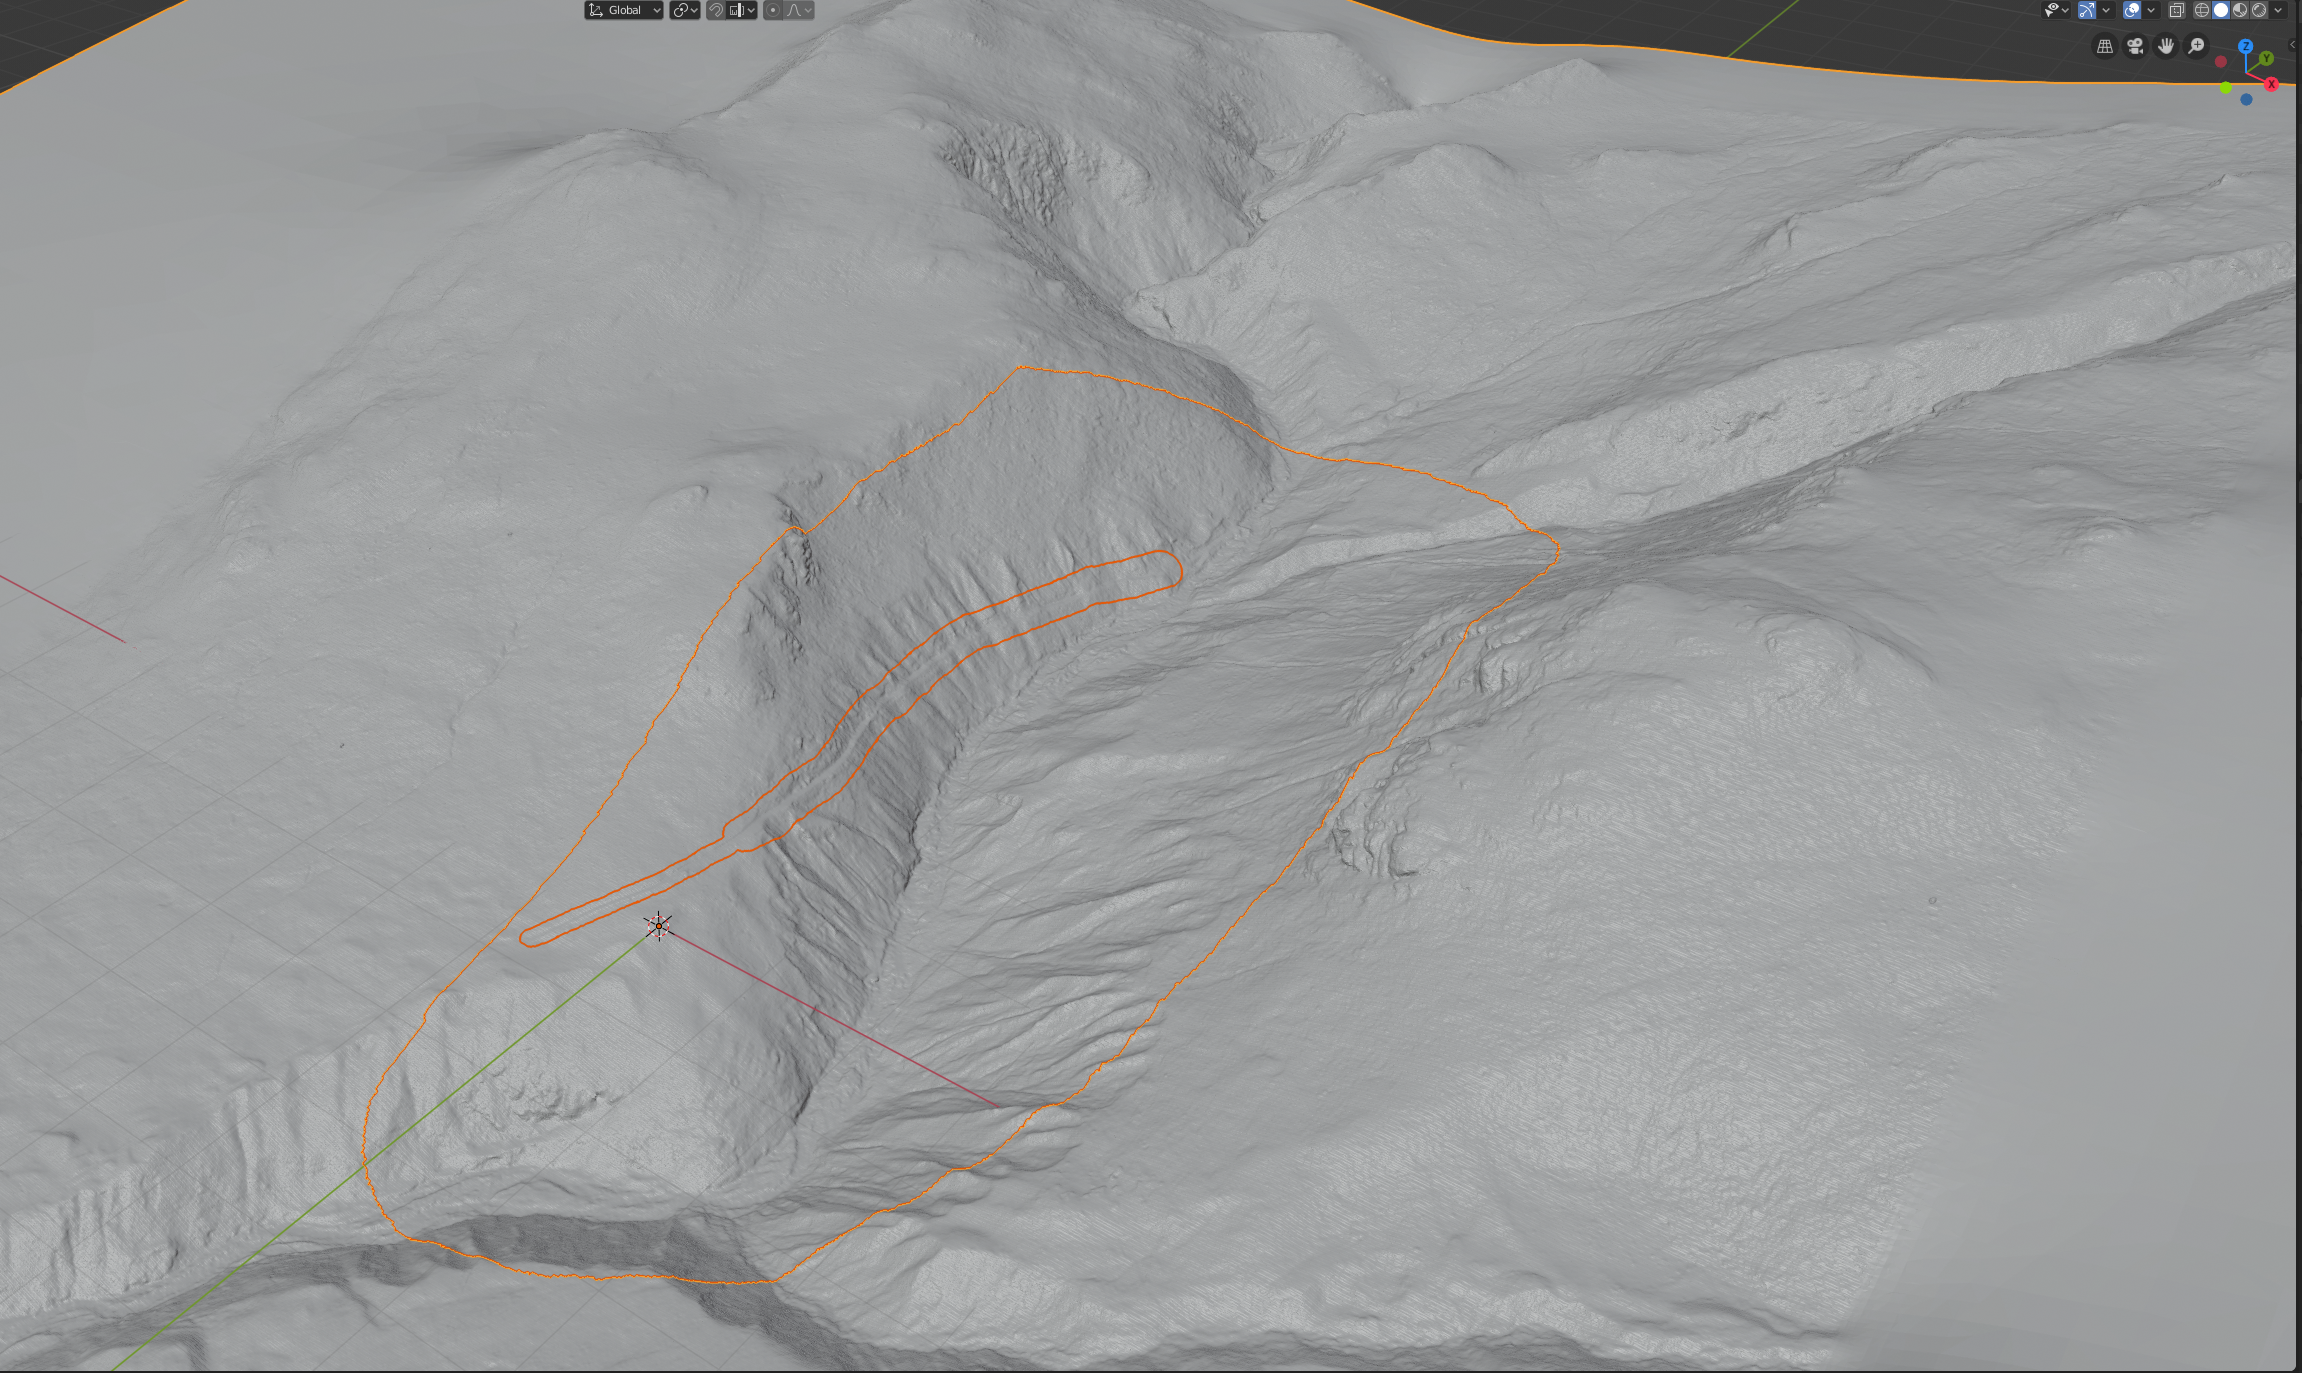
\includegraphics[width=\ImageWidth]{figures/model_original.PNG}
            \caption{Partitioning of the Model Before Simplification}
            \label{fig:model_original}
        \end{figure}
        \FloatBarrier
        
        \todo{Update partition image}
    
    \subsection{Simplify Model in Meshlab}
        With the model divided into different parts, they can be simplified tailored to their importance. The Quadratic Edge Collapse Decimation algorithm was used to achieve this. This simplification allows to preserve the general topology, as well as the edges of the final model. This is important as the different parts of the model need to fit together at the end. The simplification was controlled by stating the percentage of vertices that should survive. Different percentages was tested for the ground models, to trade off quality against file size. As the models had a very high vertex count, the walkway was scaled to 15 \% of original vertex count, the main area was set to 2 \% and the rest were set to 0.1 \%.
        
        \todo{Input image of post-simplification}
    
    \subsection{Rework and Texture Model in Blender}
        Although the recreation of the walkway was successful, the omnidirectional treadmill needs more space than a person would normally need. This is because it is less precise than actual walking, as well as a little harder to control. To accommodate this the walkway was reworked in Blender to provide a flatter surface for the players. When the three ground models were ready, they were textured using a satellite image from Google Maps. Finally the ground models were exported as \texttt{.fbx} files, as Unity does not support the \texttt{.ply} format.
        
        \todo{Input image of post rework}

\section{Implementation in Unity}
    % How stuff was made in Unity, potentially code snippets.
    \subsection{Viewing Stereoscopic 360 Images}
    
    \subsection{Decorating the Game World}

\section{Achieved Milestones}
    % A table documenting achieved milestones: when and what
    To document the progress, different milestones with dates are noted in the following table:
    
    \FloatBarrier
    \begin{table}[htbp]
        \centering
        \begin{tabular}{|c|p{0.8\linewidth}|}
            \hline
            \textbf{Date} & \textbf{Milestone} \\
            \hline
            2020-01-15 & Meeting with domain experts to show progress and plans \\
            2020-02-04 & Finished ground models \\
            2020-02-06 & Meeting with domain expert to discuss interaction elements and content to be included \\
            2020-02-13 & Supervisor meeting to discuss research questions and gameplay elements \\
            2020-02-25 & \todo{User testing with geography students} \\
            2020-02-\todo{?} & \todo{Domain expert test of images} \\
            \hline
        \end{tabular}
        \caption{Achieved milestones}
        \label{tab:milestones}
    \end{table}
    \FloatBarrier
